
\documentclass[fleqn,addpoints]{exam}

\usepackage{graphicx}
\usepackage{float}
\usepackage{amsmath}
\usepackage{cancel}
\usepackage{polynom}
\usepackage{caption}

\printanswers

% \ifprintanswers \usepackage{2in1, lscape} \fi

\title{Math 115 Notes}
\date{December 14, 2010}

\begin{document}

\maketitle
 
\section{Overview}

These notes contain a summary of the information that is sort of contained in section 2.2 of the text.  I borrowed
most of this from another text book which I think is a bit clearer.

\section{Terminology}
A polynomial is a function which looks something like this: $P(x) = 2x^3 + 7x^2 - x + 17$.

Here are some terms (no pun intended) used to describe the parts of a polynomial:

\begin{description}

\item[coefficient] the coefficients are the numbers which are not powers which appear in the equation.  The coefficients
  for this example are: 2, 7, -1, and 17 

\item[leading term] the leading term is the first term, when the polynomial is written the normal way with the highest
  power first.  In this case, the leading term is $2x^3$.

\item[leading coefficient] the coefficient from the leading term.  In this case, the leading coefficient is $2$.

\item[degree] the degree is the highest power which appears in the equation.  The degree of this example is 3.

\end{description}

\section{Monomials}
A monomials is a polynomials with only one term.  Examples of monomials are: $f(x) = x^2$, $f(x) = -2x^4$, etc.  

The graph of any monomial looks generally like the graph of either $f(x) = \pm x^2$ or $f(x) = \pm x^3$.  If the degree
of the polynomial is even, the graph will look like a variation of $f(x) = x^2$ and if the degree of the polynomial is
odd, the graph will look like a variation of $f(x) = x^3$.

See figures and \ref{even} and \ref{odd} .

\begin{figure}[H]
  \centering
  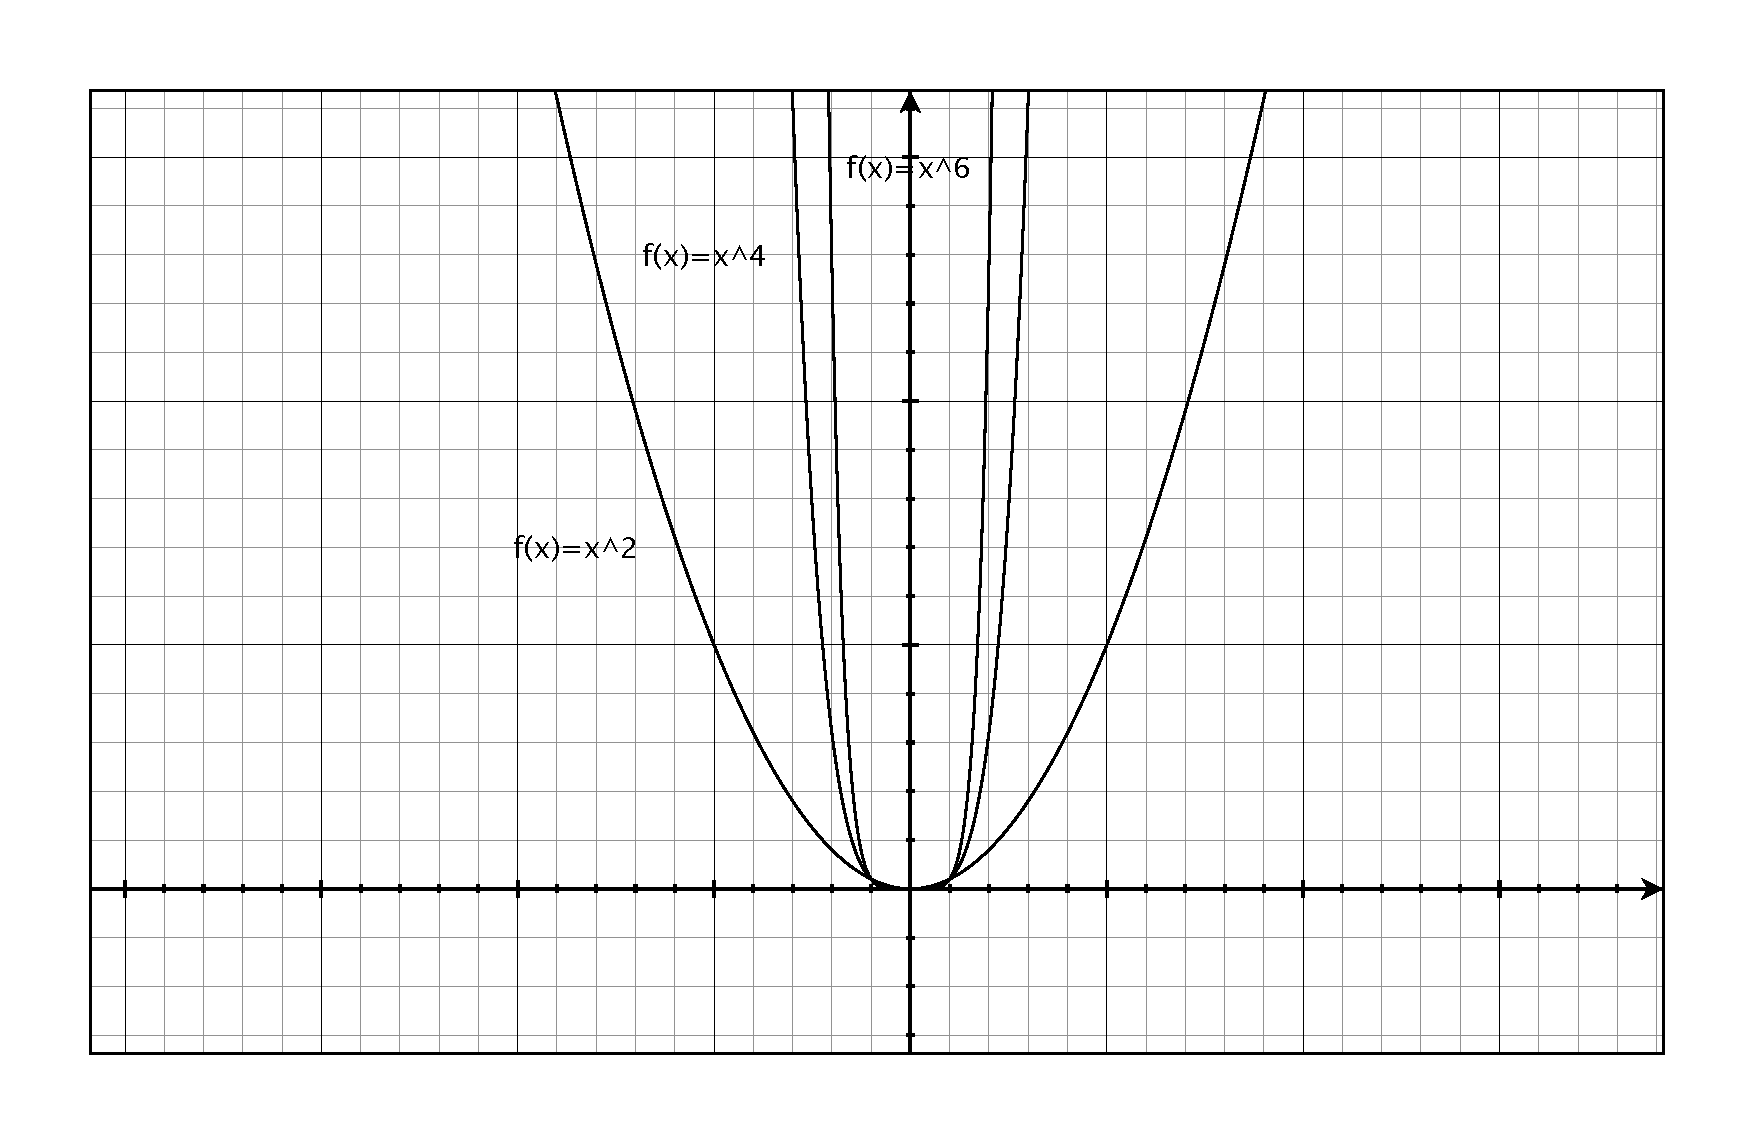
\includegraphics[width=14cm,height=10cm]{even_powered_monomials.eps}
  \caption{Even Powered Monomials}
  \label{even}
\end{figure}

\begin{figure}[H]
  \centering
  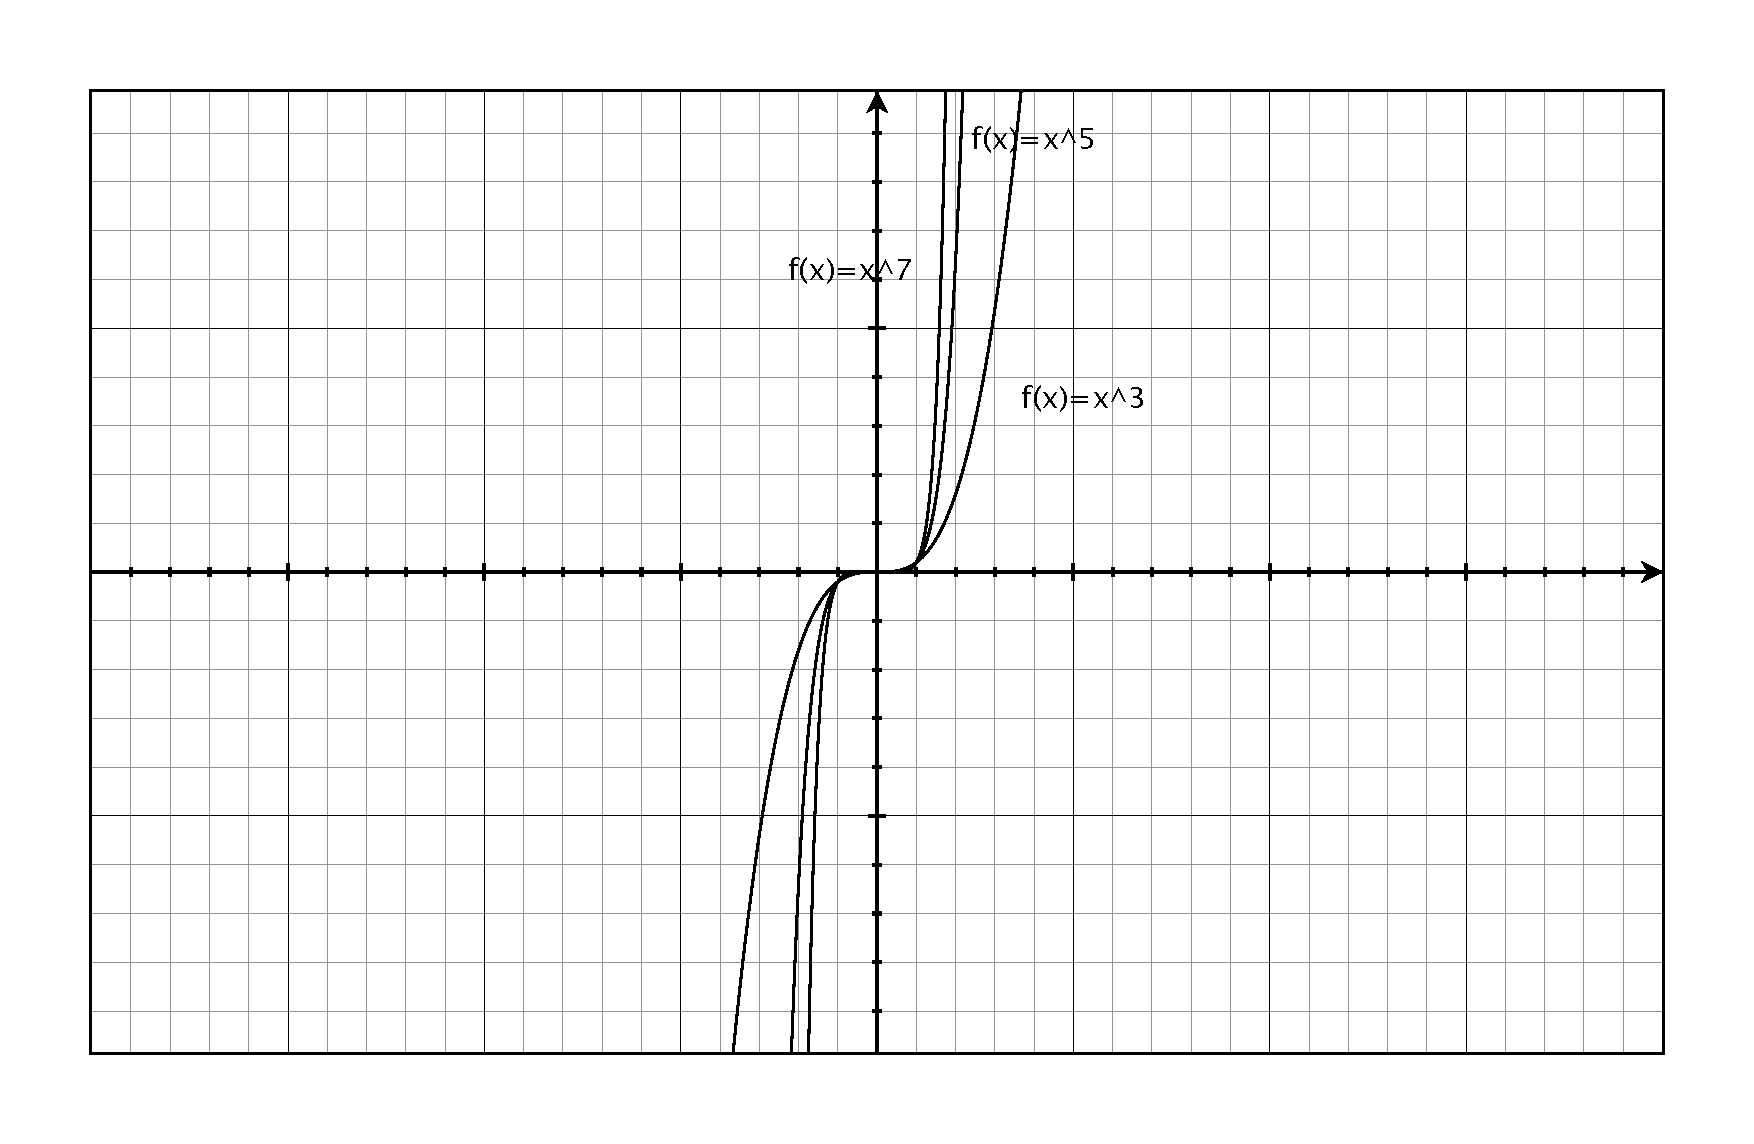
\includegraphics[width=14cm,height=10cm]{odd_powered_monomials.eps}
  \caption{Odd Powered Monomials}
  \label{odd}
\end{figure}

\section{End Behavior}
\label{end_behavior}

For values of $x$ around 0, each polynomial looks different, and you have to pay attention to the details to draw the
graph correctly.  However for large enough $x$ (or small enough negative $x$) none of the terms other than the first one
matter much.  There are four cases to consider:
\begin{enumerate}

\item If the degree is even
\begin{enumerate}
\item and the leading coefficient is positive, $f(x) \rightarrow \infty$ as $x \rightarrow \pm \infty$
\item and the leading coefficient is negative, $f(x) \rightarrow -\infty$ as $x \rightarrow \pm \infty$
\end{enumerate}

\item If the degree is odd
\begin{enumerate}
\item and the leading coefficient is positive, $f(x) \rightarrow \infty$ as $x \rightarrow \infty$ and $f(x) \rightarrow
  -\infty$ as $x \rightarrow -\infty$
\item and the leading coefficient is positive, $f(x) \rightarrow -\infty$ as $x \rightarrow \infty$ and $f(x)
  \rightarrow \infty$ as $x \rightarrow -\infty$ 
\end{enumerate}
\end{enumerate}

See figures \ref{zoom:in} and \ref{zoom:out} for the graph of the same polynomial viewed at different scales.

\begin{figure}[H]
  \centering
  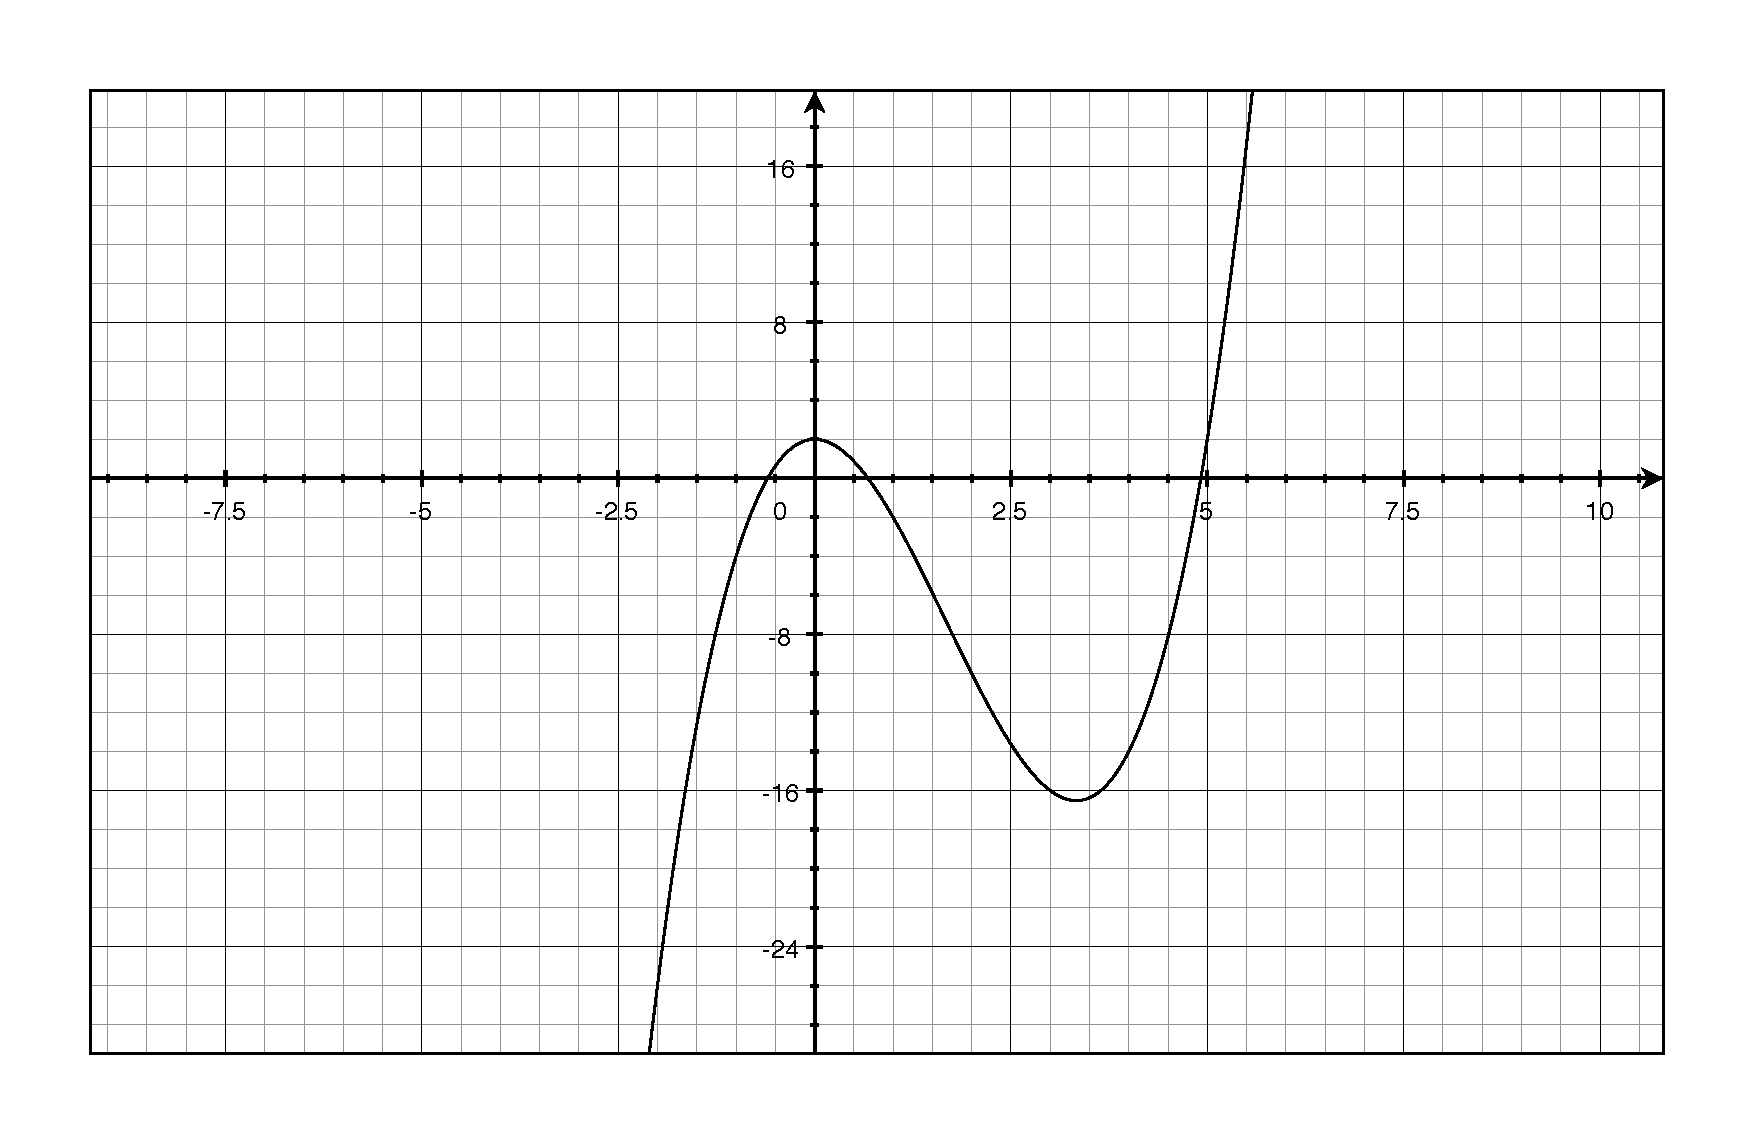
\includegraphics[width=14cm,height=10cm]{zoom_in.eps}
  \caption{$f(x) = x^3-5x^2+2$ close to the origin}
  \label{zoom:in}
\end{figure}

\begin{figure}[H]
  \centering
  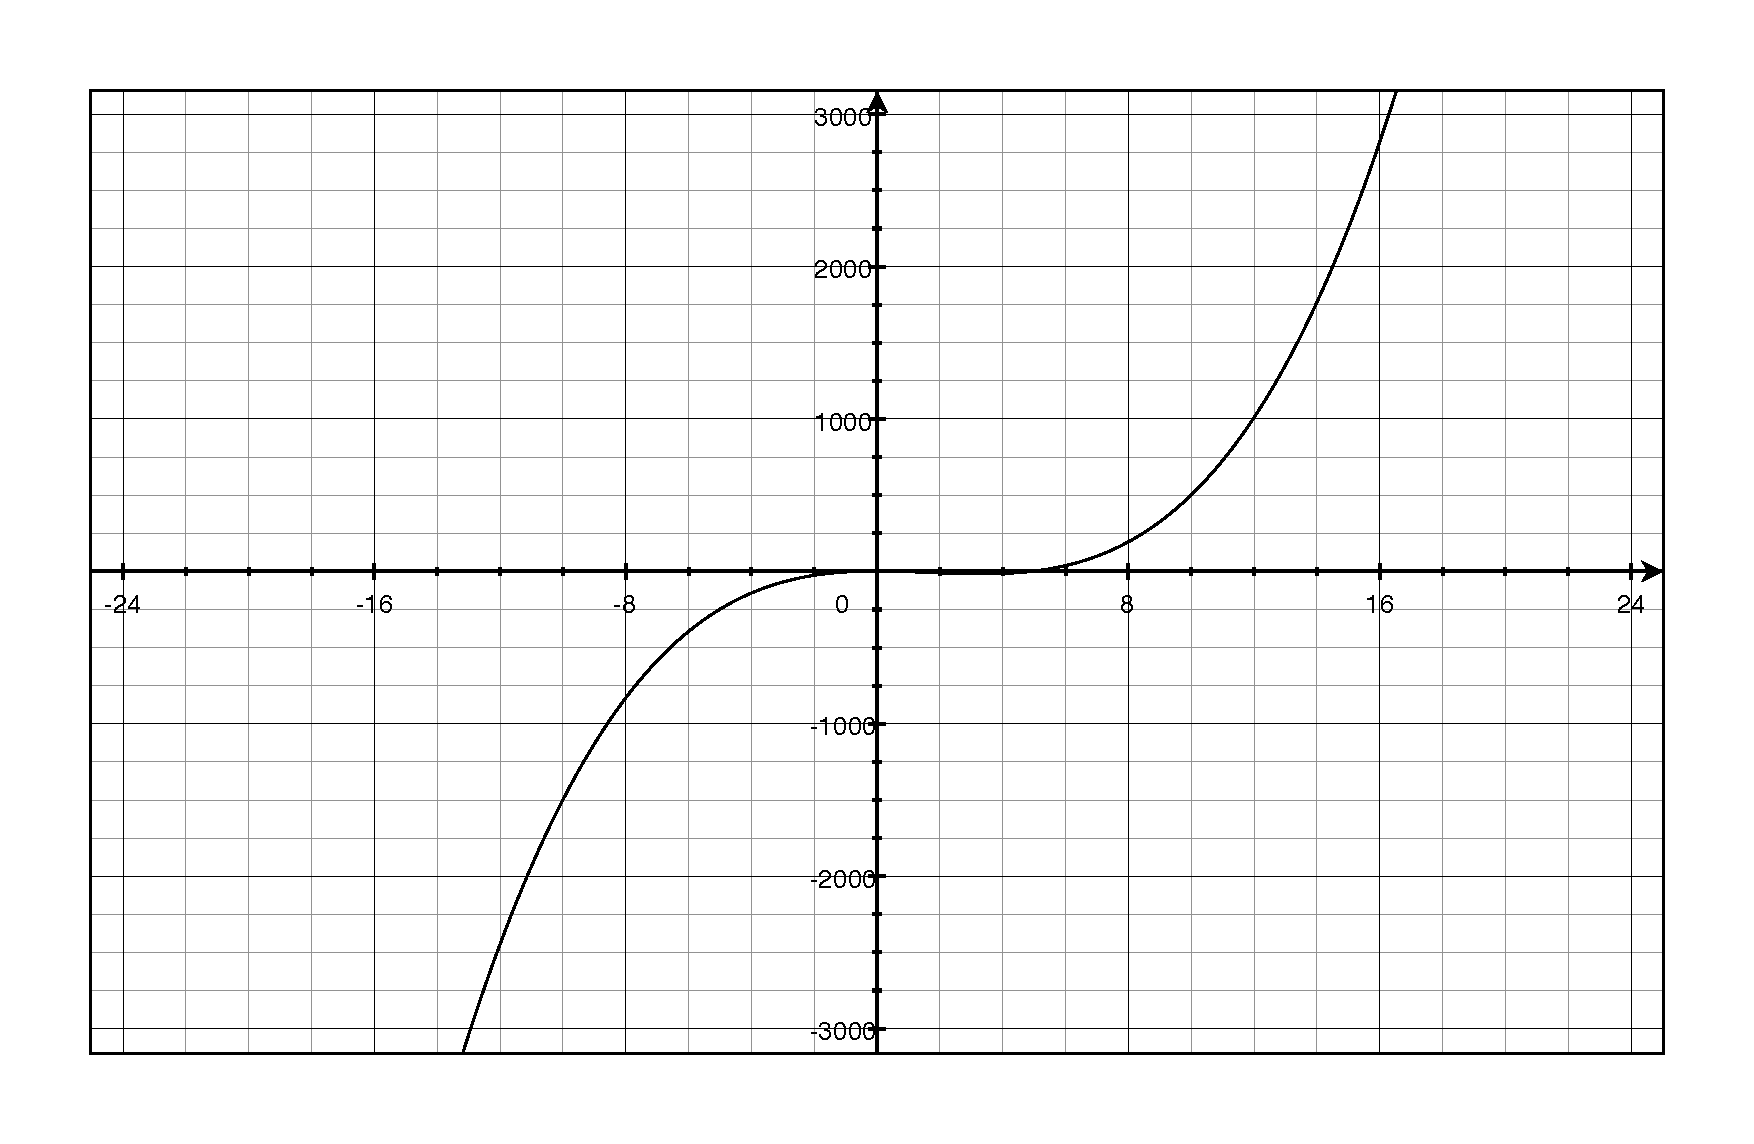
\includegraphics[width=14cm,height=10cm]{zoom_out.eps}
  \caption{$f(x) = x^3-5x^2+2$ zoomed out}
  \label{zoom:out}
\end{figure}


\section{Zeros}

The zeros are the points where the polynomial crosses the x-axis.  Other names for the zeros are {\em roots} and 
{\em x-intercepts}.  You can find the zeros by setting the polynomial equal to zero and solving for $x$.  And you solve for
$x$ in using the same approach you used in math 113--factor and and find the numbers which make each factor equal to
zero.

\section{Local Extrema}
{\em Extrema} is, I think, the plural of the Latin word for {\em extreme}.  A graph's {\em local extrema} are all of its
local minimums and local maximums (see below).

\begin{description}
\item[local minimum] A local minimum is a valley in the graph.  If you look at other values of $x$ near a local minimum, you'll find that the
value for $f(x)$ for all of them is a bit bigger than the the value at the local minimum.

\item[local maximum] A local maximum is a hill in the graph.  If you look at other values of $x$ near a local maximum, you'll find that the
value for $f(x)$ for all of them is a bit smaller than the the value at the local maximum.
\end{description}

Graphs may have more than one local minimum or local maximum.  But there is a limit on the number you can expect.  A
polynomial of degree $n$ will have at most $n-1$ local extrema.  For example, a $5^{th}$ degree polynomial will have no
more than 4 local extrema.

\section{Graphing}

\subsection{Procedure}
Armed with all this information, you are now ready to graph polynomials.  The general procedure is:
\begin{enumerate}

\item Look at the degree and leading of the polynomial.  This tells you whether the final graph will look roughly like $f(x) = \pm
  x^2$ (even degree) or $f(x) = \pm x^3$ (odd degree).

\item Find the zeros by setting the polynomial equal to zero and factoring.  This gives you all the places where the
  graph will cross the x-axis.

\item Select some test points between the roots.  This gives you a few additional points and tells you whether the graph
  is above or below the x-axis in this region.  Include $x=0$ as one of your test points, so that you will know what the
  y-intercept is.

\item Draw the graph.
\end{enumerate}

\subsection{Example}

As an example, lets draw the graph of $f(x) = -x^3 + 2x^2 + 3x$.

\begin{enumerate}

\item The polynomial is degree 3 and the leading coefficient is negative, so the final graph will look basically like $f(x) = -x^3$

\item To find the zeros:
\begin{align*}
  -x^3 + 2x^2 + 3x &= 0 \\
  x^3 - 2x^2 - 3x &= 0 \\
  x(x^2 - 2x - 3) &= 0 \\
  x(x-3)(x+1) &= 0 \\
\end{align*}

So the zeros are at: $x = {-1, 0, 3}$

\item
Try a few test points:
\begin{itemize}
  \item $f\left( -\dfrac{1}{2} \right) = \dfrac{1}{8} + \dfrac{1}{2} -\frac{3}{2} = -\dfrac{7}{8}$
  \item $f(1) = -1+2+3 = 4$
  \item $f(2) = -8 + 8 + 6 = 6$
\end{itemize}

\item Draw the graph.  See Figure \ref{example}.
\end{enumerate}

\begin{figure}[H]
  \centering
  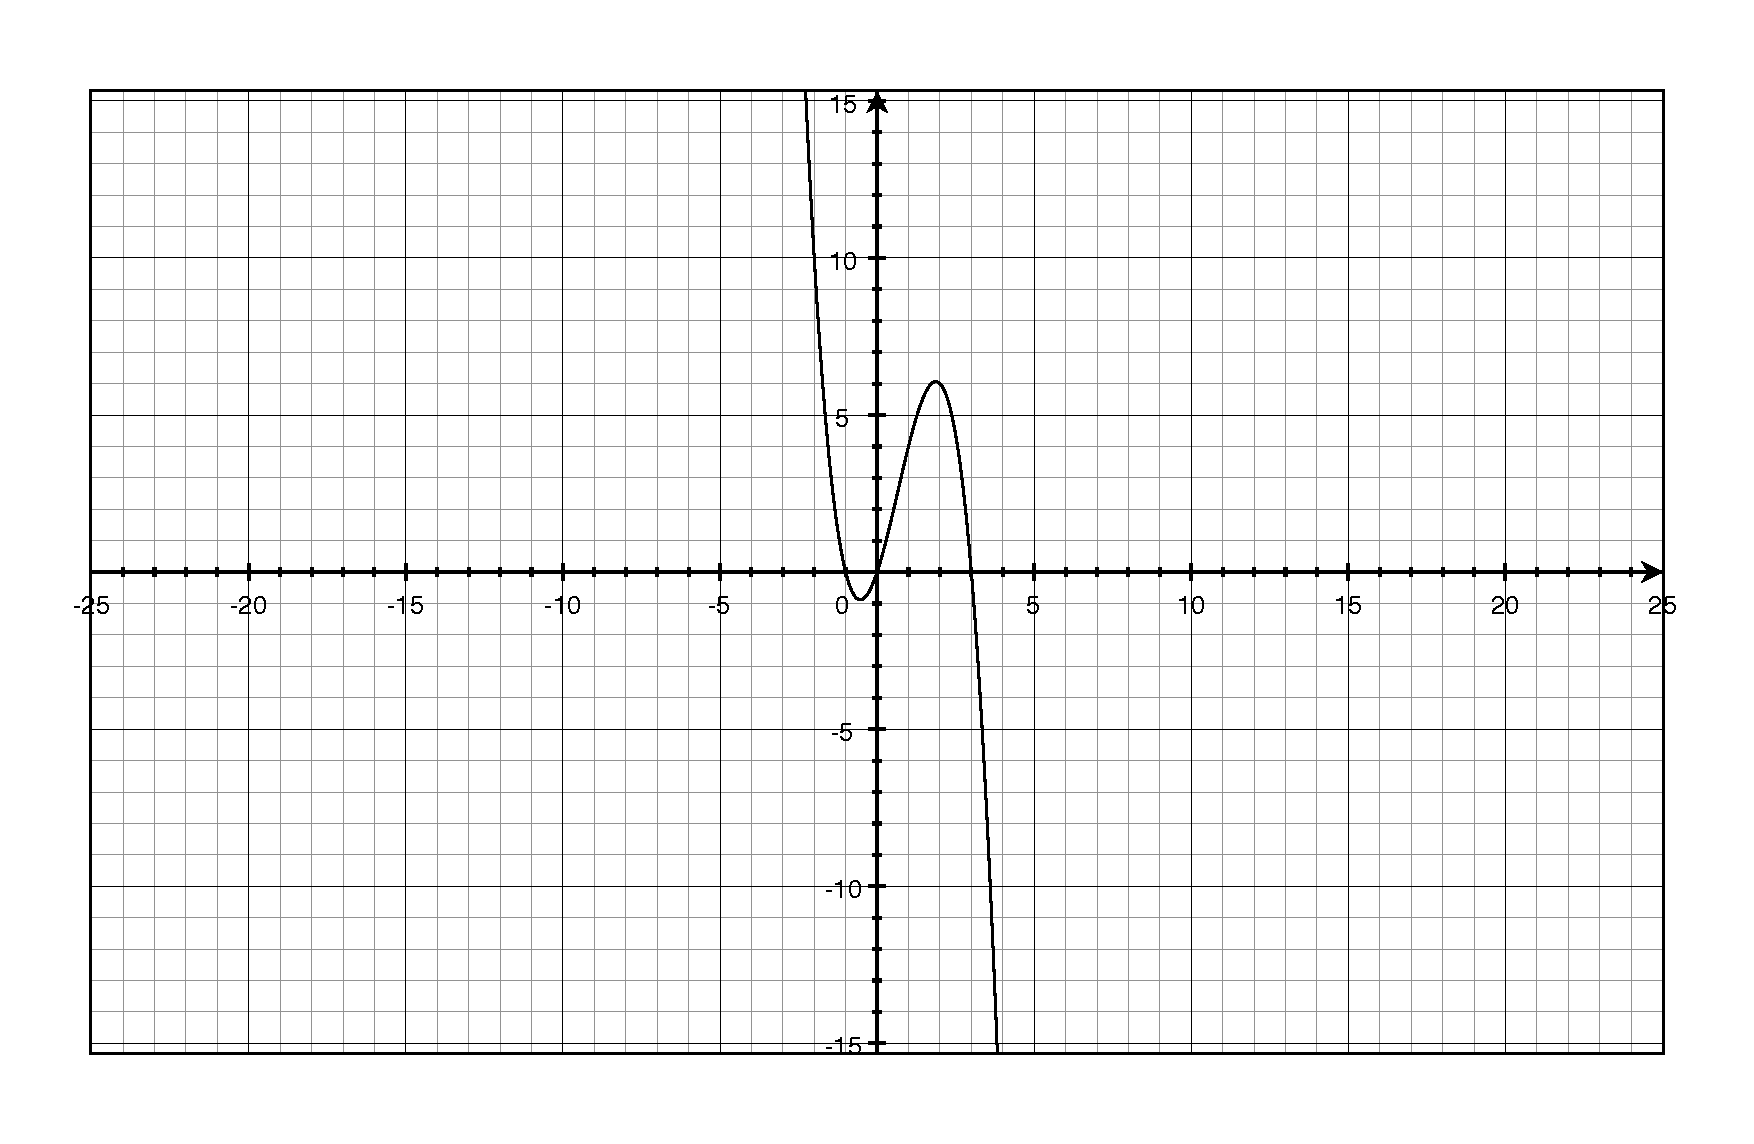
\includegraphics[width=14cm,height=10cm]{example.eps}
  \caption{$f(x) = -x^3 + 2x^2 + 3x$}
  \label{example}
\end{figure}


 
\end{document}

